\documentclass{beamer}

\usepackage{graphicx}

\input{../../../../texmacros/commands.tex}

\DeclareMathOperator*{\argmax}{argmax}

\usetheme{Madrid}

\begin{document}

\setlength{\parskip}{1em}
    
\begin{frame}
    \title{Linear Smoothers II}
    \subtitle{\texttt{numpy 101}; binary classification; kernel smoothers; density estimation}
    \date{DATA 607 --- Session 2 --- 27/02/2019}
    \maketitle
\end{frame}


\begin{frame}{\textsc{Session Plan}}
    \begin{enumerate}
        \item \texttt{numpy} 101
        \begin{itemize}
            \item axes; universal functions; broadcasting
            \item exercise
        \end{itemize}
        \item nonparametric binary classification
        \begin{itemize}
            \item decision functions
            \item zero-one loss; misclassification rate
            \item examples/demos (\texttt{sklearn})
        \end{itemize}
        \item kernel regression and classification
        \begin{itemize}
            \item kernel functions; examples
            \item Nadaraya-Watson smoothers
            \item examples/demos (\texttt{sklearn})
        \end{itemize}
        \item density estimation
        \begin{itemize}
            \item histogram estimators
            \item kernel estimators
            \item connection with kernel regression and classification
        \end{itemize}
        \item summatory exercise
    \end{enumerate}   
\end{frame}

\begin{frame}{\textsc{1.} \texttt{numpy} \textsc{101}}
    
    \begin{center}
        \texttt{numpy\_101.ipynb}
    \end{center}
\end{frame}



\begin{frame}{\textsc{Regression with categorical response}}
    \textbf{Setting:}
    \begin{itemize}
        \item two \emph{classes} with \emph{labels} $0$ and $1$
        \item $(X, Y)$ jointly distributed, $X\in\RR^n$, $Y\in\{0,1\}$
        \item $L(\hat y, y)$ a \emph{loss function}
    \end{itemize}

    \textbf{Goal:}
    Find a function
    \[
        \hat{r}:\RR^n\longrightarrow \RR
    \]
    that minimizes the average risk:
    \[
        \EE\big[ L(\hat r(X), Y)\big]
    \]
    $L(\hat f(X), Y)$ is the penalty for predicting $\hat f(X)$ when the target was $Y$.
\end{frame}

\begin{frame}{\textsc{Example: Na\"ive Bayes Classifier}}

    Let $L$ is \emph{zero-one loss}:
    \[
        L(\hat y, y) = \begin{cases}
            0&\text{if $\hat y = y$,}\\
            1&\text{if $\hat y \neq y$}
        \end{cases}
    \]
    The average risk, $\EE\big[ L(\hat r(X), Y)\big]$, is minimized by the \emph{Bayes estimator}:
    \[
        \hat f(x) := \argmax_{y\in\{0,1\}}P(X=x|Y=y)P(Y=y)
    \]

    This is not so useful if we don't know $P(x, y)$!
\end{frame}

\begin{frame}{\textsc{$K$-nearest neighbors classifier}}
    Suppose $K$ is odd.

    Let $\hat r$ be the nearest neighbors regressor associated to the dataset
    \[
        (X_1, Y_1),\ldots, (X_n, Y_n).
    \]
    Since $Y_i\in\{0,1\}$, we have $\hat r(x)\in \left\{\frac0K, \frac1K,\ldots, \frac KK\right\}$ for all $x$.
    
    Let
    \[
        \hat f(x) := \text{$\hat r(x)$, rounded to the nearest integer}.
    \]
\end{frame}

\begin{frame}{\textsc{2. Kernel Regression}}
    {\large\textsc{$K$-nearest neighbors as a kernel smoother}}
    Let
    \[
        K_k(x, x_i) = \begin{cases}
            1&\text{if $x_i$ is one of the $k$-nearest neighbors of $x$}\\
            0&\text{otherwise.}
        \end{cases}
    \]
    \begin{align*}
        \hat r_k(\vx) &= \frac1k\sum_{i=1}^n K_k(x, x_i)Y_i\\
        &= \frac{\sum_{i=1}^n K_k(x, x_i)Y_i}{\sum_{i=1}^n K(x, x_i)}
    \end{align*}
\end{frame}

\begin{frame}{{\large{\textsc{Local averaging as a kernel smoother}}}}
    Let
    \[
        K_h(x, x_i) = \begin{cases}
            1&\text{if $\|x - x_i\|\leq h$}\\
            0&\text{otherwise.}
        \end{cases}
    \]
    \[
        \hat r_h(x) = \frac{\sum_{i=1}^n K_h(x, x_i)Y_i}{\sum_{i=1}^n K_h(x, x_i)} 
    \]
    If
    \[
        K(x) = \One_{[-1, 1]}(x) = \begin{cases}
            1&\text{ if $x\in[-1, 1]$,}\\
            0&\text{otherwise,}
        \end{cases}
    \]
    then
    \[
        K_h(x, x_i) = K\left(\frac{x - x_i}h\right)
    \]
    and
    \[
        \hat r_h(x) = \frac{\sum_{i=1}^n K\left(\frac{x - x_i}h\right)Y_i}
        {\sum_{i=1}^n K\left(\frac{x - x_i}h\right)} 
        \]
\end{frame}

\begin{frame}{{\large{\textsc{Kernel functions and Nadaraya-Watson smoothers}}}}
    \begin{block}{Definition}
    A \emph{kernel function} is a function $K(x)$ such that
    \begin{enumerate}
        \item $K(x)\geq 0$,
        \item $K(-x) = K(x)$,
        \item $\displaystyle{\int_{-\infty}^\infty K(x)dx = 1}$,
    \end{enumerate}
    \end{block}

    \begin{block}{Definition}
        The \emph{Nadaraya-Watson smoother} with bandwidth $h>0$ associated to the kernel function $K(x)$
        and the dataset $(x_1, Y_1),\ldots,(x_n, Y_n)$ is
        \[
            \hat r_h(x) = \frac{\sum_{i=1}^n K\left(\frac{x - x_i}h\right)Y_i}
            {\sum_{i=1}^n K\left(\frac{x - x_i}h\right)} 
        \]
    \end{block}
\end{frame}

\begin{frame}{{\large{\textsc{Examples of kernels}}}}
\begin{enumerate}
    \item The \emph{boxcar kernel}:
    \[
        K(x) = \frac12\One_{[-1, 1]}(x)
    \]
    \item The \emph{Gaussian kernel}:
    \[
        K(x) = \frac1{\sqrt{2\pi}}e^{-x^2/2}
    \]
    \item The \emph{Epanechnikov kernel}:
    \[
        K(x) = \frac34(1-x^2)\One_{[-1, 1]}(x)
    \]
\end{enumerate}
The Nadaraya-Watson smoother associated to the boxcar kernel is the local average smoother.
\end{frame}

\begin{frame}{}
    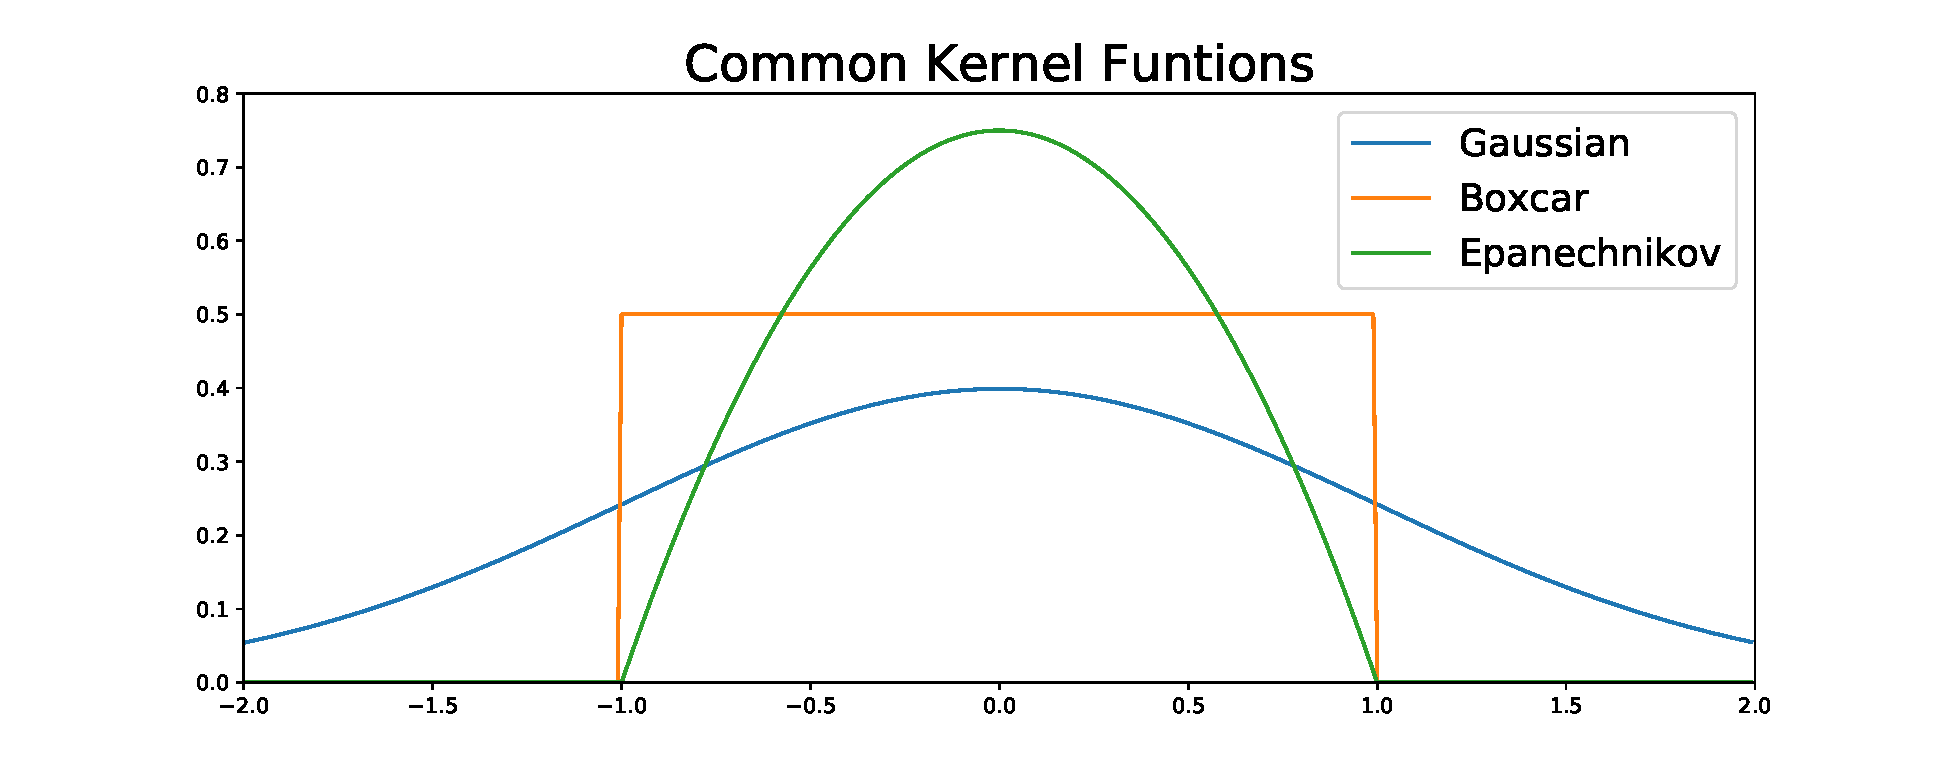
\includegraphics[scale=0.36]{kernels.pdf}
\end{frame}

\begin{frame}{}
    \begin{center}
        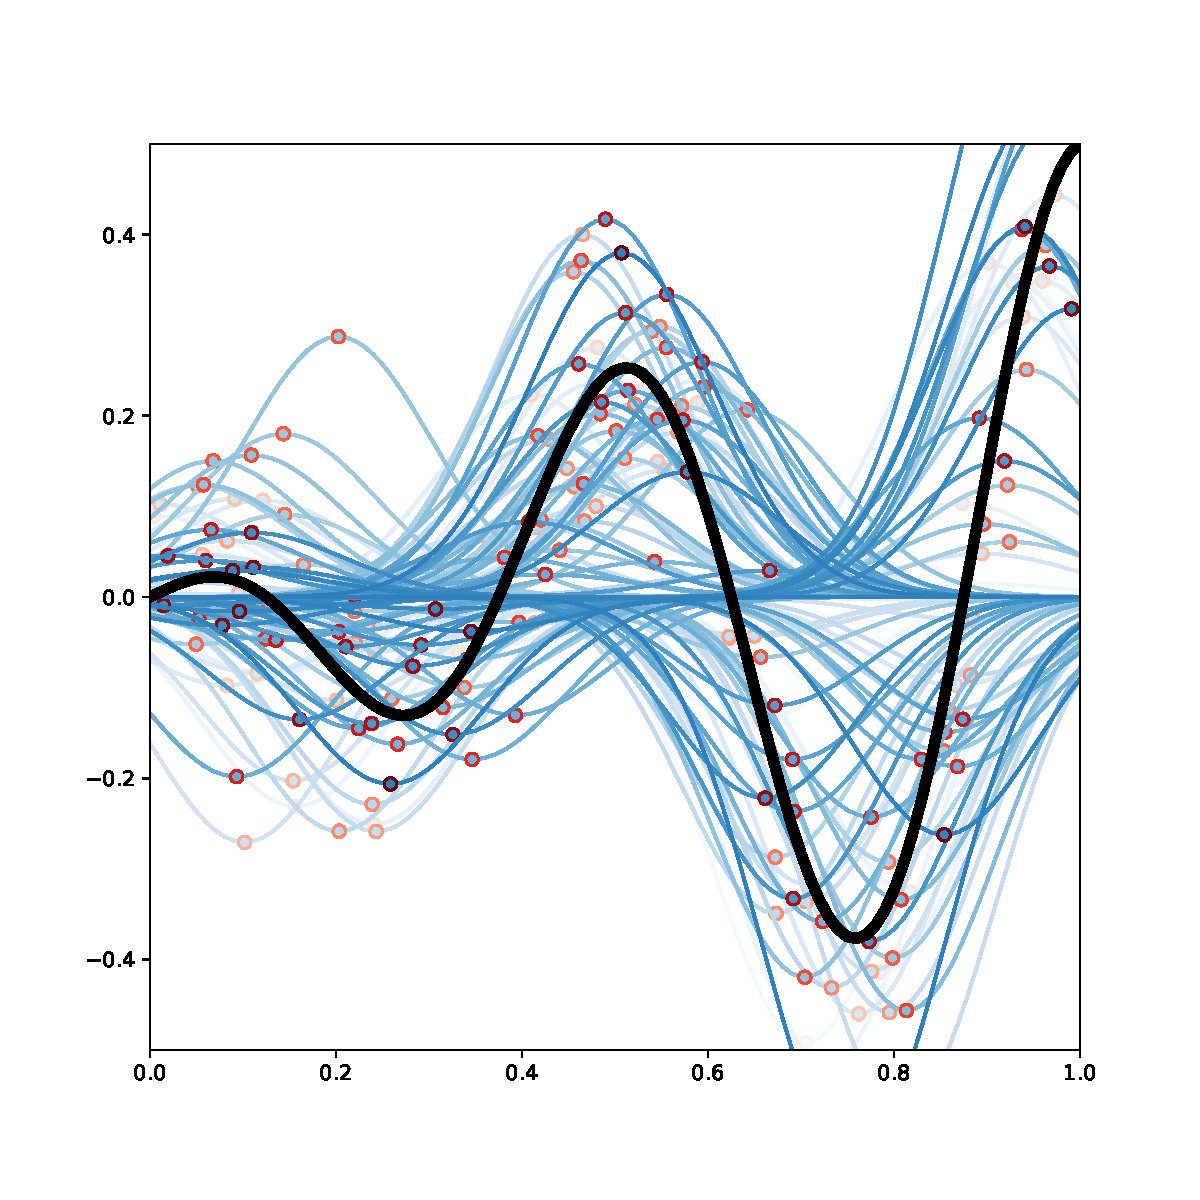
\includegraphics[scale=0.42]{waves.pdf}
    \end{center}
\end{frame}

\begin{frame}{\textsc{4. Kernel density estimation}}
    You can use kernels to estimate probability density functions.

    \begin{block}{Definition}
        The \emph{kernel density estimator} associated to a kernel function 
        $K(x)$, a bandwidth $h>0$, and a dataset $X_1,\ldots,X_n$ is
        \[
            \hat f_n(x) = \frac1{nh}\sum_{i=1}^n K\left(\frac{x - X_i}h\right).
        \]
    \end{block}
\end{frame}

\begin{frame}{{\large{\textsc{Cross validation}}}}
    To determine the optimal $h$, minimize the cross validation score.
    \begin{block}{Definition}
        The \emph{leave one out cross validation score} associated to a kernel density
        estimator $\hat f_n$ with bandwidth $h$ is
        \[
            \hat R(h) := \int\hat f_n(x)^2\,dx - \frac2n\sum_{i=1}^n\hat f_n^{(-i)}(X_i)
        \]
    \end{block}
\end{frame}
\end{document}